\begin{frame}{Hard spheres and colloids}
	\begin{textblock*}{0.6\textwidth}(10mm,88mm)
		\simplephasediagram{}%
	\end{textblock*}
	The volume fraction $\phi$ is like an inverse temperature.
	\bigskip
	\def\svgwidth{\textwidth}\input{phase_diagram.pdf_tex}
	
	\bigskip
	Well approximated by sterically stabilised colloids\\
	\begin{footnotesize}\citet{pusey1987ogt}\end{footnotesize}
\end{frame}

\tikzsetnextfilename{sem_hist}
\begin{frame}{Our colloids}
	\begin{columns}
	\column{0.5\textwidth}
	\begin{center}
	\rotatebox{90}{\qquad \small{SEM image}}\includegraphics[width=0.8\columnwidth, height=0.6\columnwidth]{SEM}
	\end{center}
	\structure{Solvent}
	\begin{itemize}
		\item Cis-decalin
		\item Cyclohexylbromide
	\end{itemize}
	Matching
	\begin{itemize}
		\item Optical index
		\item Density (with $T$ control)
	\end{itemize}
	\column{0.5\textwidth}
	\begin{block}{PMMA particles}
		\begin{itemize}
			\item $\sigma \simeq \SI{3.3}{\micro\metre}$
			\item $\Delta \simeq 6\%$ not Gaussian
		\end{itemize}
		Hard spheres
		\begin{itemize}
			\item Sterically stabilized
			\item Salt to screen charges\\ (Debye length $<\SI{100}{\nano\metre}$)
		\end{itemize}
	\end{block}
	\begin{tikzpicture}
		\begin{axis}[%
			width=\columnwidth, height=0.6\columnwidth,%
			ybar,%
			ymin=0, ylabel={Size distribution},%
			xlabel={Sizes [\si{\micro\metre}]}
			]
		\usebeamercolor{palette primary}
		\addplot[ybar interval, fill=fg!50!white] file {SEM_size_distrib.txt};
		\end{axis}
	\end{tikzpicture}
	\end{columns}
\end{frame}

\tikzsetnextfilename{confocal}
\begin{frame}{Confocal microscopy}
	\begin{center}\begin{columns}[c]
	\column{0.4\textwidth}
	\begin{tikzpicture}[
		font=\footnotesize, 
		decoration={markings, mark=between positions 0.1 and 1 step 0.2\columnwidth with {\arrow{stealth}}},
	]
	\draw[thick] (-0.12\columnwidth,0) -- (-0.012\columnwidth,0) (0.012\columnwidth,0) -- (0.12\columnwidth,0);
	\node[left] at (-0.12\columnwidth,0) {aperture};
	\fill[name path=dichro, cyan, rotate around={-45:(0,-0.35\columnwidth)}]  (-0.2\columnwidth,-0.34\columnwidth) rectangle (0.2\columnwidth,-0.36\columnwidth) (0, -0.34\columnwidth) node[above, black, rotate=-45] {beam splitter};
	\draw[thick] (-0.35\columnwidth,-0.23\columnwidth) -- (-0.35\columnwidth,-0.348\columnwidth) (-0.35\columnwidth,-0.362\columnwidth) -- (-0.35\columnwidth,-0.47\columnwidth);
	\node[above] at (-0.35\columnwidth,-0.23\columnwidth) {pinhole};
	\fill[cyan] (0, -\columnwidth) arc (-90:-70:0.6\columnwidth) node (lensright) {} 
		arc (70:110:0.6\columnwidth) node (lensleft) {}
		arc (-110:-90:0.6\columnwidth);
	\path[name path=lensbottom] (lensleft) arc (-110:-70:0.6\columnwidth);
	\path[name path=lenstop] (lensright) arc (70:110:0.6\columnwidth);
	\fill[orange] (-0.15\columnwidth, -1.05\columnwidth) rectangle (0.15\columnwidth, -1.15\columnwidth);
	\draw[dashed] (-0.2\columnwidth, -1.08\columnwidth) -- (0.2\columnwidth, -1.08\columnwidth);
	\node[left] at (-0.2\columnwidth, -1.08\columnwidth) {focal plane};
	\node[above] at (0,0.1\columnwidth) {light source};
	\path[name path=iray1] (0.012\columnwidth, 0.1\columnwidth) -- (-0.12\columnwidth, -\columnwidth);
	\path[name path=iray2] (0, -1.08\columnwidth) -- (-0.15\columnwidth, -0.95\columnwidth);
	\path[name path=iray3] (-0.012\columnwidth, 0.1\columnwidth) -- (0.12\columnwidth, -\columnwidth);
	\path[name path=iray4] (0, -1.08\columnwidth) -- (0.15\columnwidth, -0.95\columnwidth);
	\draw[
		postaction={decorate}, green!80!black,
		name intersections={of=iray1 and dichro, by=x},
		name intersections={of=iray3 and dichro, by=y},
		]
		(0.012\columnwidth, 0.1\columnwidth) -- (x)
		(-0.012\columnwidth, 0.1\columnwidth) -- (y);
		
	\draw[
		postaction={decorate}, green!80!black, dashed, dash pattern=on 5pt off 5pt, dash phase=0pt,
		name intersections={of=iray1 and dichro, by=x}, 
		name intersections={of=iray1 and lenstop, by=a}, 
		name intersections={of=iray2 and lensbottom, by=b},
		name intersections={of=iray4 and lensbottom, by=c},
		name intersections={of=iray3 and lenstop, by=d},
		name intersections={of=iray3 and dichro, by=y},
		] 
		(x) -- (a) -- (b) -- (0, -1.08\columnwidth)
		(y) -- (d) -- (c) -- (0, -1.08\columnwidth);
	\draw[postaction={decorate}, red!80!black, 
		name intersections={of=iray1 and dichro, by=x}, 
		name intersections={of=iray3 and dichro, by=y},
		] 
		(x) -- (-0.41\columnwidth, -0.362\columnwidth) 
		(y) -- (-0.41\columnwidth, -0.348\columnwidth);
	\draw[postaction={decorate}, red!80!black, dashed, dash pattern=on 5pt off 5pt, dash phase=10pt,
		name intersections={of=iray1 and dichro, by=x}, 
		name intersections={of=iray1 and lenstop, by=a}, 
		name intersections={of=iray2 and lensbottom, by=b},
		name intersections={of=iray4 and lensbottom, by=c},
		name intersections={of=iray3 and lenstop, by=d},
		name intersections={of=iray3 and dichro, by=y},
		] 
		(0, -1.08\columnwidth) -- (b) -- (a) -- (x) 
		(0, -1.08\columnwidth) -- (c) -- (d) -- (y);
	\draw[thick, blue] (-0.39\columnwidth, -0.33\columnwidth) arc (90:270:0.025\columnwidth);
	\node[above left, rotate=90] at (-0.39\columnwidth, -0.33\columnwidth) {light detector};
	\path[name path=badray1] (0,0) -- (-0.18\columnwidth, -1.1\columnwidth);
	\path[name path=badray2] (0, -1.12\columnwidth) -- (-0.3\columnwidth, -0.85\columnwidth);
	\path[name path=badray3] (0,0) -- (0.18\columnwidth, -1.1\columnwidth);	
	\path[name path=badray4] (0, -1.12\columnwidth) -- (0.3\columnwidth, -0.85\columnwidth);
	\draw[dotted,
		name intersections={of=badray1 and dichro, by=x}, 
		name intersections={of=badray1 and lenstop, by=a}, 
		name intersections={of=badray2 and lensbottom, by=b},
		name intersections={of=badray4 and lensbottom, by=c},
		name intersections={of=badray3 and lenstop, by=d},
		name intersections={of=badray3 and dichro, by=y},
		] 
		(0, -1.12\columnwidth) -- (b) -- (a) -- (x) --  (-0.35\columnwidth, -0.38\columnwidth)
		(0, -1.12\columnwidth) -- (c) -- (d) -- (y) --  (-0.35\columnwidth, -0.33\columnwidth);
	\end{tikzpicture}
	\column{0.5\textwidth}
	\tikzsetnextfilename{confocal_slices}
	\begin{tikzpicture}
	\matrix[matrix of nodes, ampersand replacement=\&, nodes={anchor=center}]
	{
		$XY$ slice \& 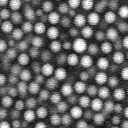
\includegraphics[width=0.5\columnwidth]{sliceXY} \\
		$XZ$ slice \& 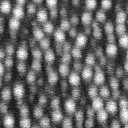
\includegraphics[width=0.5\columnwidth]{sliceXZ} \\
	};
	\end{tikzpicture}
	\end{columns}\end{center}
\end{frame}

\begin{frame}<3>{Particle tracking}
	\begin{columns}
	\column{0.6\textwidth}
	\only<1|handout:0>{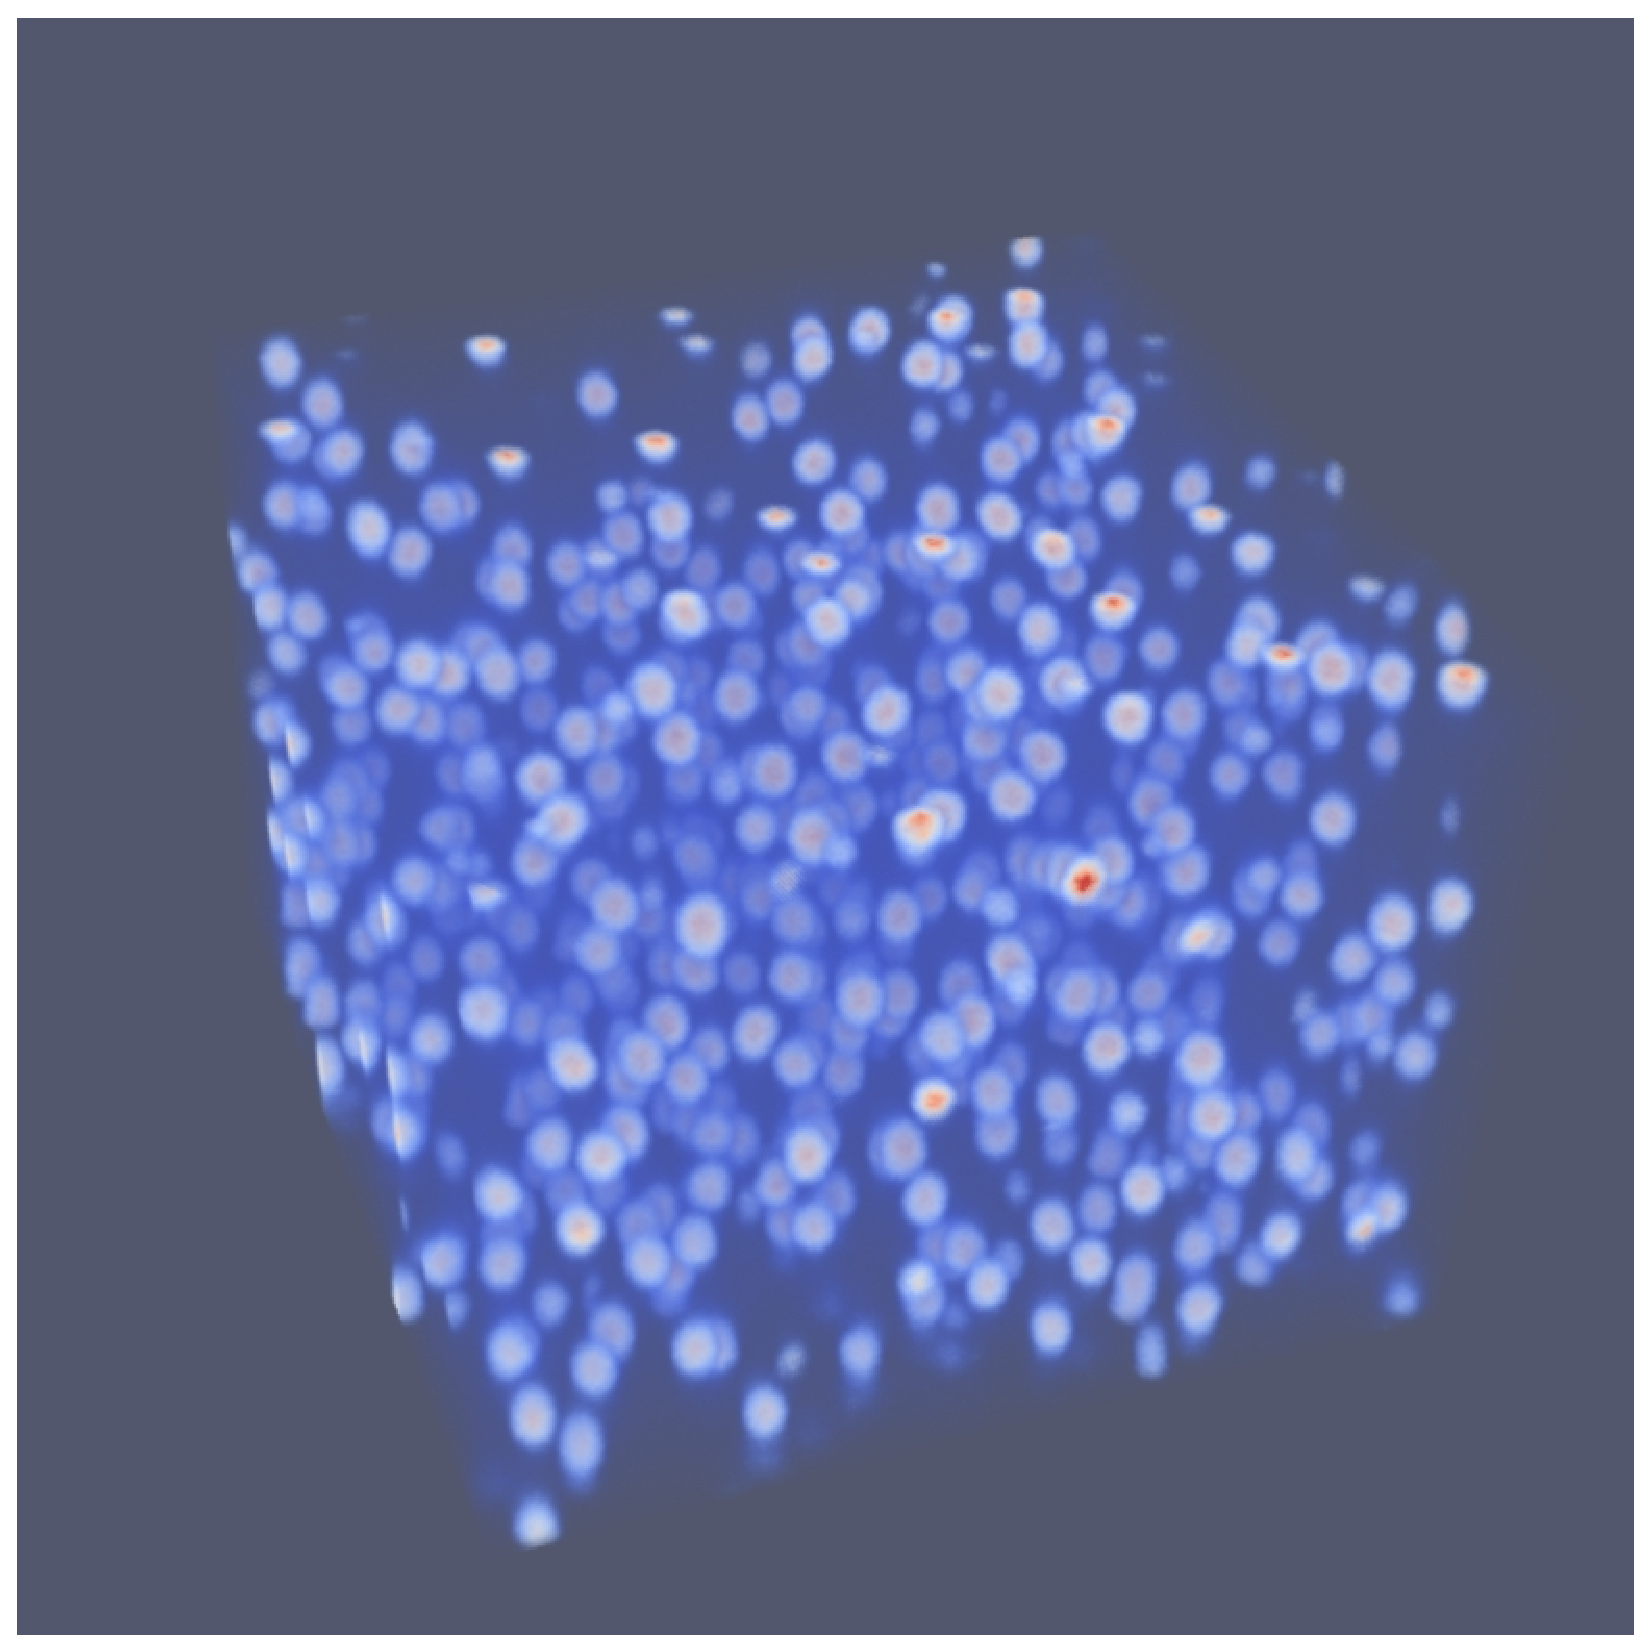
\includegraphics[width=\columnwidth]{compare_image_tracked3D_0}}%
	\only<2|handout:0>{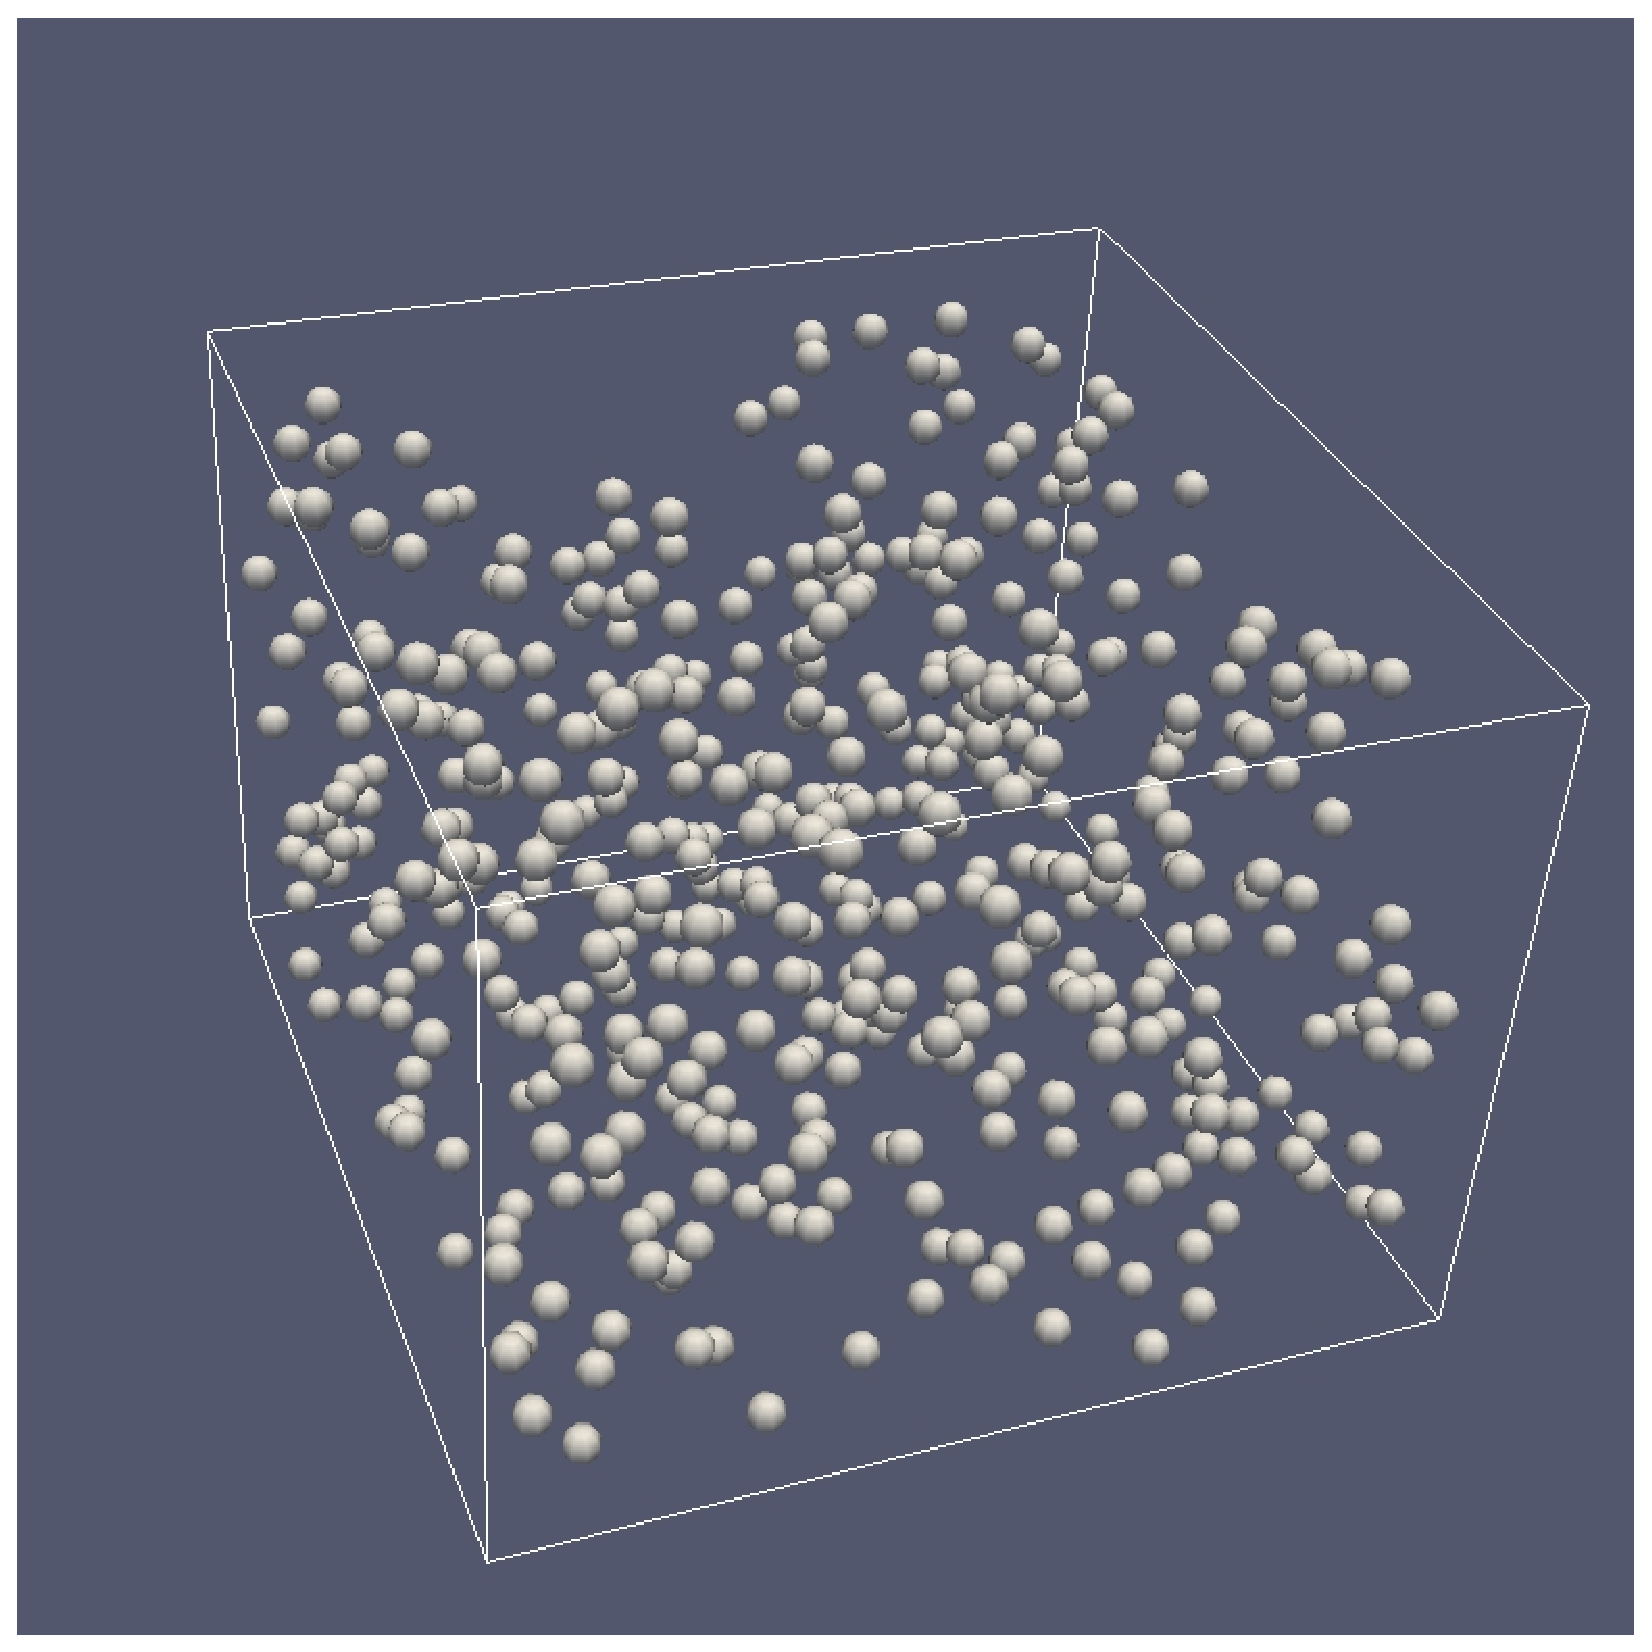
\includegraphics[width=\columnwidth]{compare_image_tracked3D_1}}%
	\only<3>{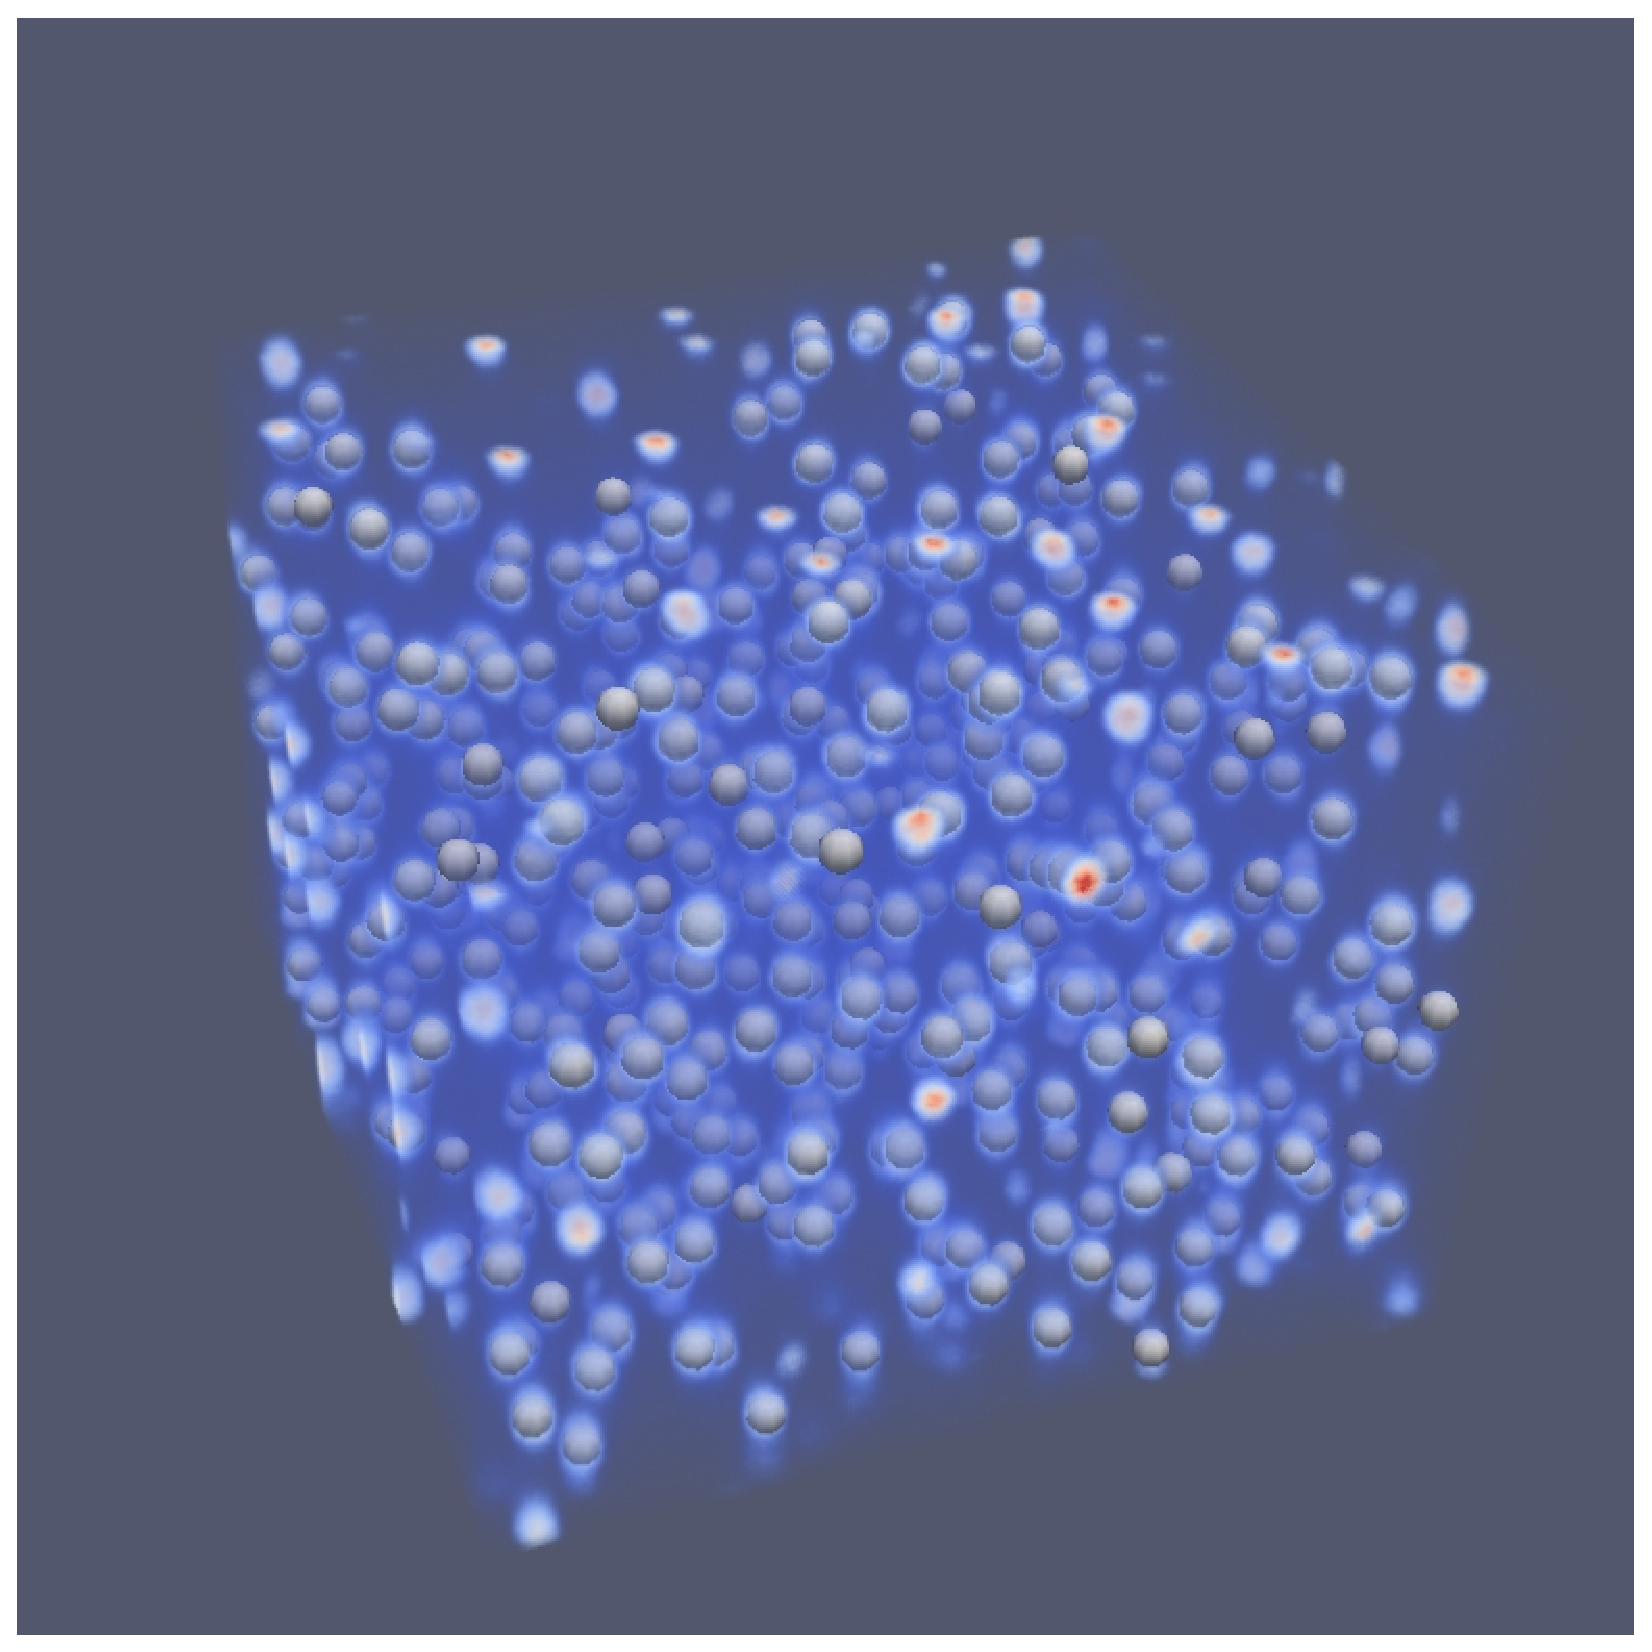
\includegraphics[width=\columnwidth]{compare_image_tracked3D_2}}\\
	\centering{\uncover<1,3>{Image}\uncover<3>{ $+$ }\uncover<2,3>{Tracked}}
	\column{0.4\textwidth}
	\footnotesize{\citet{Crocker1996}}	
	
	\bigskip
	
	\begin{itemize}
		\item All particles are tracked
		\item Only particles are tracked
		\item Coordinates are known within\\
			$\SI{0.1}{pixels} \approx \sigma/100 \approx \SI{30}{\nano\metre}$
		\item \alert{new}: arbitrary size distribution
		\item \alert{new}: sizes measured \emph{in situ}
	\end{itemize}
	\end{columns}
\end{frame}


\tikzsetnextfilename{hist_SEM_vs_multiscale}
\begin{frame}{Multiscale tracking}
	\centering
	\begin{tikzpicture}
	\begin{axis}[%
		name=hist2,
		width=0.8\columnwidth, height=0.6\columnwidth,%
		xmin=1, xmax=5,
		ylabel={Size distribution},
		ymin=0, yticklabel=\empty, ylabel near ticks,%
		legend style={legend pos=north west},
		no marks,%
		]
		\addplot[ybar, ybar interval, area legend, gray!50, fill=gray!50] file {SEM_size_distrib.txt} \closedcycle;
		\legend{\textsc{sem}}
		\addplot+[blue,dashed] table[x expr ={2*\thisrow{r}}, y expr ={5.5*\thisrow{all}}] {all_ico_icongb_mrco_X.rdist};
		\addlegendentry{In situ};
		\addplot+[red] table [x expr ={2*\thisrow{r}/1.25}, y expr ={5.5*\thisrow{all}}] {all_ico_icongb_mrco_X.rdist};
		\addlegendentry{In situ*0.8};
		\draw[->, ultra thick] (axis cs:3.15,3) -- (axis cs: 3.9, 3) node[midway, above] {swelling};%
	\end{axis}
	\end{tikzpicture}%
	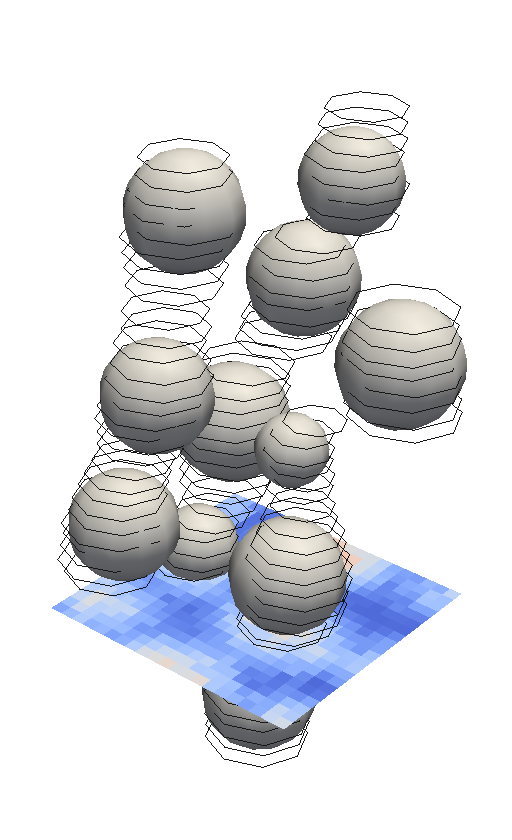
\includegraphics[width=0.2\columnwidth]{comp2D3D_crop}
	
	{\footnotesize Leocmach \& Tanaka \textit{Soft Matter} 9, 1447--1457 (2013).}
\end{frame}


\begin{frame}{Glassy dynamics}
	\begin{textblock*}{0.6\textwidth}(10mm,88mm)
		\simplephasediagram{}%
	\end{textblock*}
	From the tracked trajectories
	\tikzsetnextfilename{glassy_dynamics}%
	\begin{tikzpicture}
		\pgfplotsset{fitc/.style={solid, no markers, forget plot, domain=1:1e4}}
		\pgfplotsset{every axis/.append style={width=0.48\textwidth}}
		\pgfplotsset{cycle list name=grade5}
		\begin{axis}[%
			at={(0,0)},
			height=0.33\textwidth, %
			xlabel=$t/\tau_B$, xmode=log,%
			ylabel=\sffamily{Self ISF}, ymin=0,%
			legend style={at={(0,-0.5)}, anchor=north west},
			reverse legend,
			]
			\addplot+[fitc] {0.943 * exp(-(x/4.60)^0.72)};
			\addplot+[only marks] file {LS3954.isf};
			\addplot+[fitc] {0.901 * exp(-(x/10.78)^0.72)};
			\addplot+[only marks] file {LS4446.isf};
			\addplot+[fitc] {0.894 * exp(-(x/15.51)^0.70)};
			\addplot+[only marks] file {LS4582.isf};
			\addplot+[fitc] {0.876 * exp(-(x/60.18)^0.60)};
			\addplot+[only marks] file {LS5079.isf};
			\addplot+[fitc] {0.787 * exp(-(x/2408.)^0.70)};
			\addplot+[only marks] file {go1.isf};
			\addlegendimage{legend image code/.code={\node[right] {$\phi\;\pm$};}};
			\legend{$0.497$, $0.535$, $0.540$, $0.555$, $0.575$, $0.003$};
		\end{axis}
		\pgfplotsset{fitc/.style={no markers, forget plot, domain=0.3:3}}
		\begin{semilogxaxis}[%
			at={(0.49\textwidth,0)},
			height=0.33\textwidth, %
			xlabel=$t/\tau_B$,%
			xmin=1, xmax=1e4,%
			ylabel=$\alpha_2(t)$,%
			only marks,%
			]
			\addplot file {LS3954.ngp};
			\addplot file {LS4446.ngp};
			\addplot file {LS4582.ngp};
			\addplot file {LS5079.ngp};
			\addplot file {go1.ngp};
		\end{semilogxaxis}
		\pgfplotsset{cycle list name=black white}
		\tikzset{every mark/.append style={scale=1.2}}
		\begin{axis}[%
			at={(0.49\textwidth,-0.3\textwidth)},
			height=0.33\textwidth, %
			xlabel=$\phi$,%
			xtick={0.5,0.52,...,0.6},%
			ylabel=$\tau_\alpha/\tau_B$, ymode=log, %
			cycle list={{black, mark=*},{black, mark=square}},%
			]
			\addplot+[mark=none, forget plot, domain=0.49:0.58] {exp(0.28970401*x/(0.59841615-x))};
			\addplot+[only marks] table[x index=0, y index=1]{xi_phi.dat};
			\addplot+[only marks, every mark/.append style={draw=gray, scale=1.2}] table[x index=0, y index=4]{xi_phi.dat};
			\node at (rel axis cs:0,1) (a) {};
		\end{axis}
	\end{tikzpicture}
\end{frame}


\begin{frame}{Dynamic heterogeneities}
\begin{textblock*}{0.6\textwidth}(10mm,88mm)
		\simplephasediagram{}%
	\end{textblock*}
\begin{columns}
	\column{0.4\textwidth}
	Slow particles
	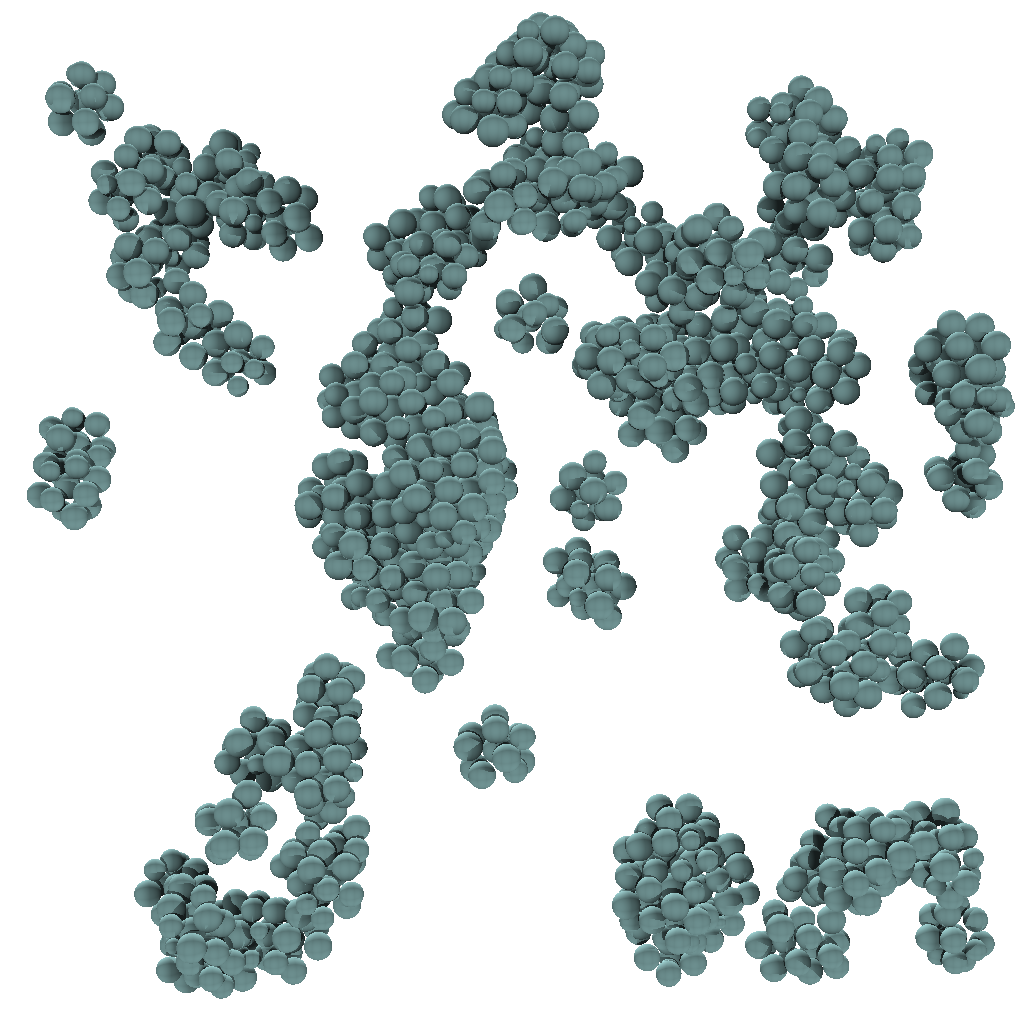
\includegraphics[width=\columnwidth]{cgsd_2tau.png}
	\column{0.6\textwidth}
	\tikzsetnextfilename{dynhet}%
	\begin{tikzpicture}
		\begin{loglogaxis}[%
			anchor=outer south,
			title={Four-point structure factor},
			width=0.9\textwidth,
			height=0.5\textwidth, %
			xlabel={$q\xi_4$}, ylabel={$S_4(q)/\chi_4$},
			cycle list name=grade5,%
			xmin=0.25, xmax=5, ymin=0.05,%
			xtick={0.5, 1, 2, 4},
			xticklabel=\pgfmathparse{exp(\tick)}%
				\pgfmathprintnumber{\pgfmathresult},
			%legend pos=south west, reverse legend,
			]
			\addplot+[only marks] table[x expr={\thisrowno{0}*0.703}, y expr={\thisrowno{1}/0.634}] {LS3954.S4};
			\addplot+[only marks] table[x expr={\thisrowno{0}*0.804}, y expr={\thisrowno{1}/0.744}] {LS4446.S4};
			\addplot+[only marks] table[x expr={\thisrowno{0}*0.835}, y expr={\thisrowno{1}/0.778}] {LS4582.S4};
			\addplot+[only marks] table[x expr={\thisrowno{0}*1.017}, y expr={\thisrowno{1}/1.011}] {LS5079.S4};
			\addplot+[only marks] table[x expr={\thisrowno{0}*1.959}, y expr={\thisrowno{1}/2.950}] {go1.S4};
			\addplot+[black, no markers, forget plot, domain=0.3:3] {1/(1+x^2)};
		\end{loglogaxis}
		\pgfplotsset{cycle list name=black white}
		\tikzset{every mark/.append style={scale=1.2}}
		\begin{axis}[%
			anchor=outer north,
			title={Growing dynamic length scale},
			%at={(0.1\textwidth,-0.6\textwidth)},
			width=0.6\textwidth, %
			xlabel=$\phi$, xmin=0.49, xmax=0.58, xlabel near ticks,%
			xtick={0.5,0.52,...,0.6},%
			ylabel=$\xi_4$, ymax=2.5,
			ytick={0.5,1,1.5,2},
			ylabel near ticks,%
			]
			\addplot+[mark=none, forget plot, domain=0.49:0.58] {0.216 * (0.6/x-1)^(-2.0/3.0)};
			\addplot+[only marks, mark=square, every mark/.append style={draw=gray, scale=1.2},] table[x index=0, y expr=\thisrowno{5}]{scale.xi};
		\end{axis}
	\end{tikzpicture}
\end{columns}
\end{frame}